\documentclass[12pt]{article}
\usepackage{geometry}
\geometry{a4paper, margin=1in}
\usepackage{booktabs}
\usepackage{tabularx}
\usepackage{float}
\usepackage{graphicx}
\usepackage{enumitem}
\usepackage{xcolor}
\usepackage{hyperref}
\hypersetup{colorlinks=true, linkcolor=blue, citecolor=blue, urlcolor=blue}

\title{Systems Requirements Specification: Privacy Preserving Data Analytics Engine (E-Privacy)}
\author{Dilmith D. L. S., Hansana O. G. V., Vidyananda H. K. H.}
\date{August 21, 2026}

\begin{document}
\maketitle

\section{Introduction}

\subsection{Purpose}
This document is a concrete requirements specification for a system that computes on encrypted data without ever decrypting it server-side.

\subsection{Scope}
The Engine allows a Data Owner (e.g. a hospital, bank or research institute) to outsource statistical aggregation of sensitive records to an untrusted cloud environment while cryptographically guaranteeing that the cloud never observes plaintext values. The scope covers functional and non-functional requirements, system architecture, data flow and the empirical justification for the selected cryptographic scheme.

\subsection{Assumptions}
These are the assumptions that were made to scope this SRS:
\begin{itemize}[leftmargin=2.5em]
    \item[A1.] The Engine targets \textbf{additive aggregate analytics} (sum, average, count, weighted average) as the primary workload, consistent with the Feasibility PoC. Complex joins, non-linear functions (e.g. median, standard deviation without a secondary protocol) are deferred to a later phase.
    \item[A2.] The \textbf{Data Owner is a single trusted entity} per deployment (e.g. one hospital) that holds the private key; multi-owner federated aggregation is a future extension requiring threshold cryptography.
    \item[A3.] The cloud provider is treated as \textbf{honest-but-curious}: it will follow the protocol correctly but will attempt to learn as much as possible from ciphertext and metadata. Active/Byzantine cloud behavior is mitigated only by the verifiable computation log, not prevented outright.
    \item[A4.] Network transport (TLS 1.3) and at-rest storage encryption (AES-256) are assumed already compliant per the organization's existing infrastructure and are treated as satisfied preconditions.
    \item[A5.] Private key material is managed and stored securely on the Data Owner side, following the organization's existing key-management practices; the Engine does not implement its own key-custody mechanism but integrates with whatever secure key store the Data Owner already operates.
\end{itemize}

\section{System Architecture}

The Engine partitions responsibility across a trusted Data Owner domain and an untrusted Cloud Analytics Engine domain, directly closing the ``Data-in-Use'' gap.

\begin{figure}[H]
    \centering
    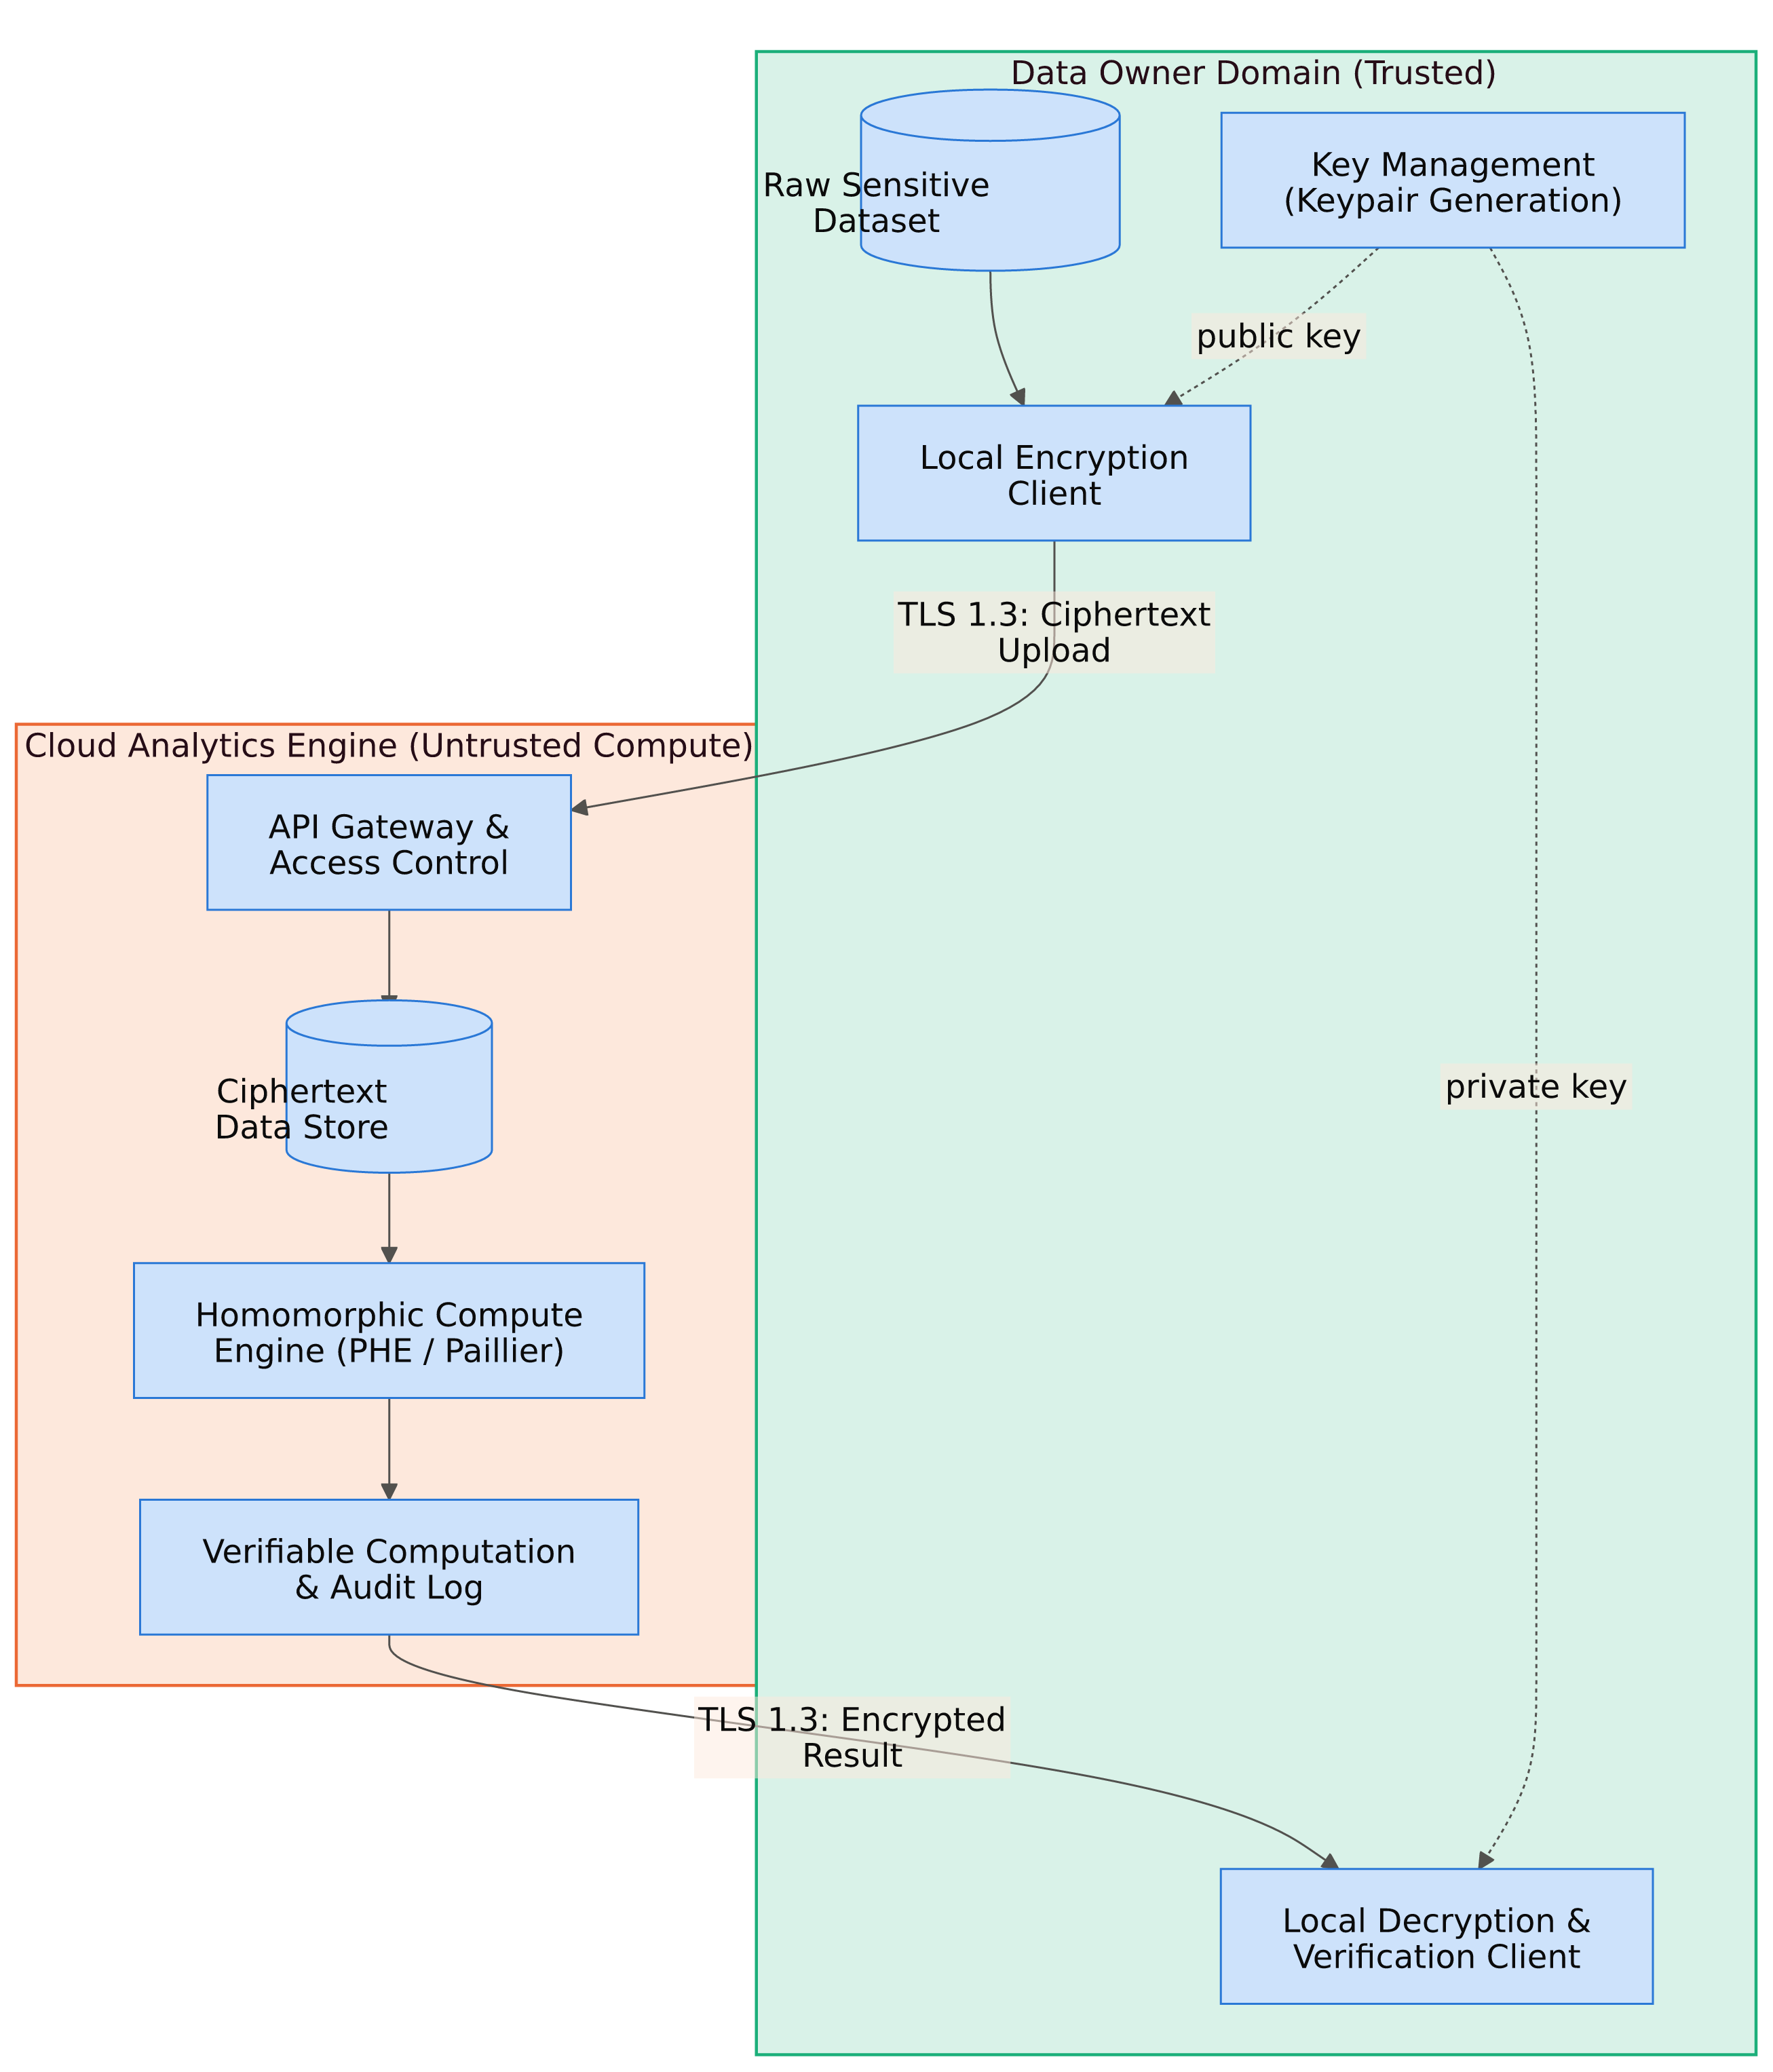
\includegraphics[width=0.95\textwidth]{sources/srs/system-architecture.png}
    \caption{High-level system architecture: encryption and decryption occur exclusively within the trusted Data Owner domain; the cloud only ever manipulates ciphertext.}
    \label{fig:sys_arch}
\end{figure}

\begin{figure}[H]
    \centering
    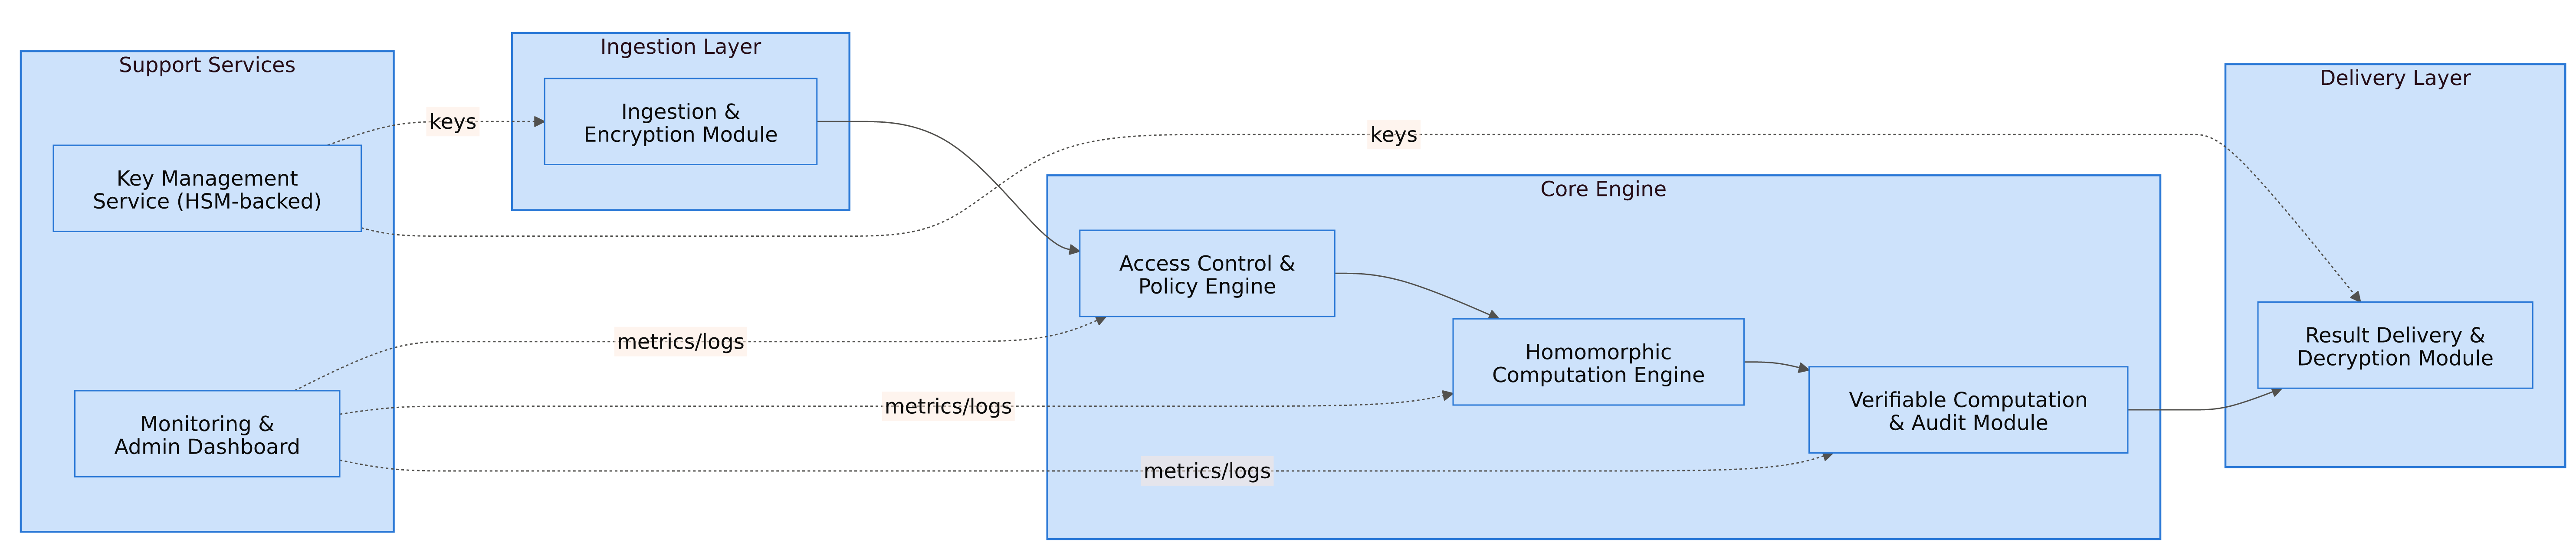
\includegraphics[width=0.95\textwidth]{sources/srs/component-breakdown.png}
    \caption{Component/module breakdown of the Engine across the ingestion, core computation, support, and delivery layers.}
    \label{fig:components}
\end{figure}

\subsection{End-to-End Data Flow}
Figure~\ref{fig:data_flow} traces a single analytics request end-to-end, showing exactly where the private key is used (only within the Data Owner domain, steps 1--2 and 9--10) and where the cloud only ever handles ciphertext.

\begin{figure}[H]
    \centering
    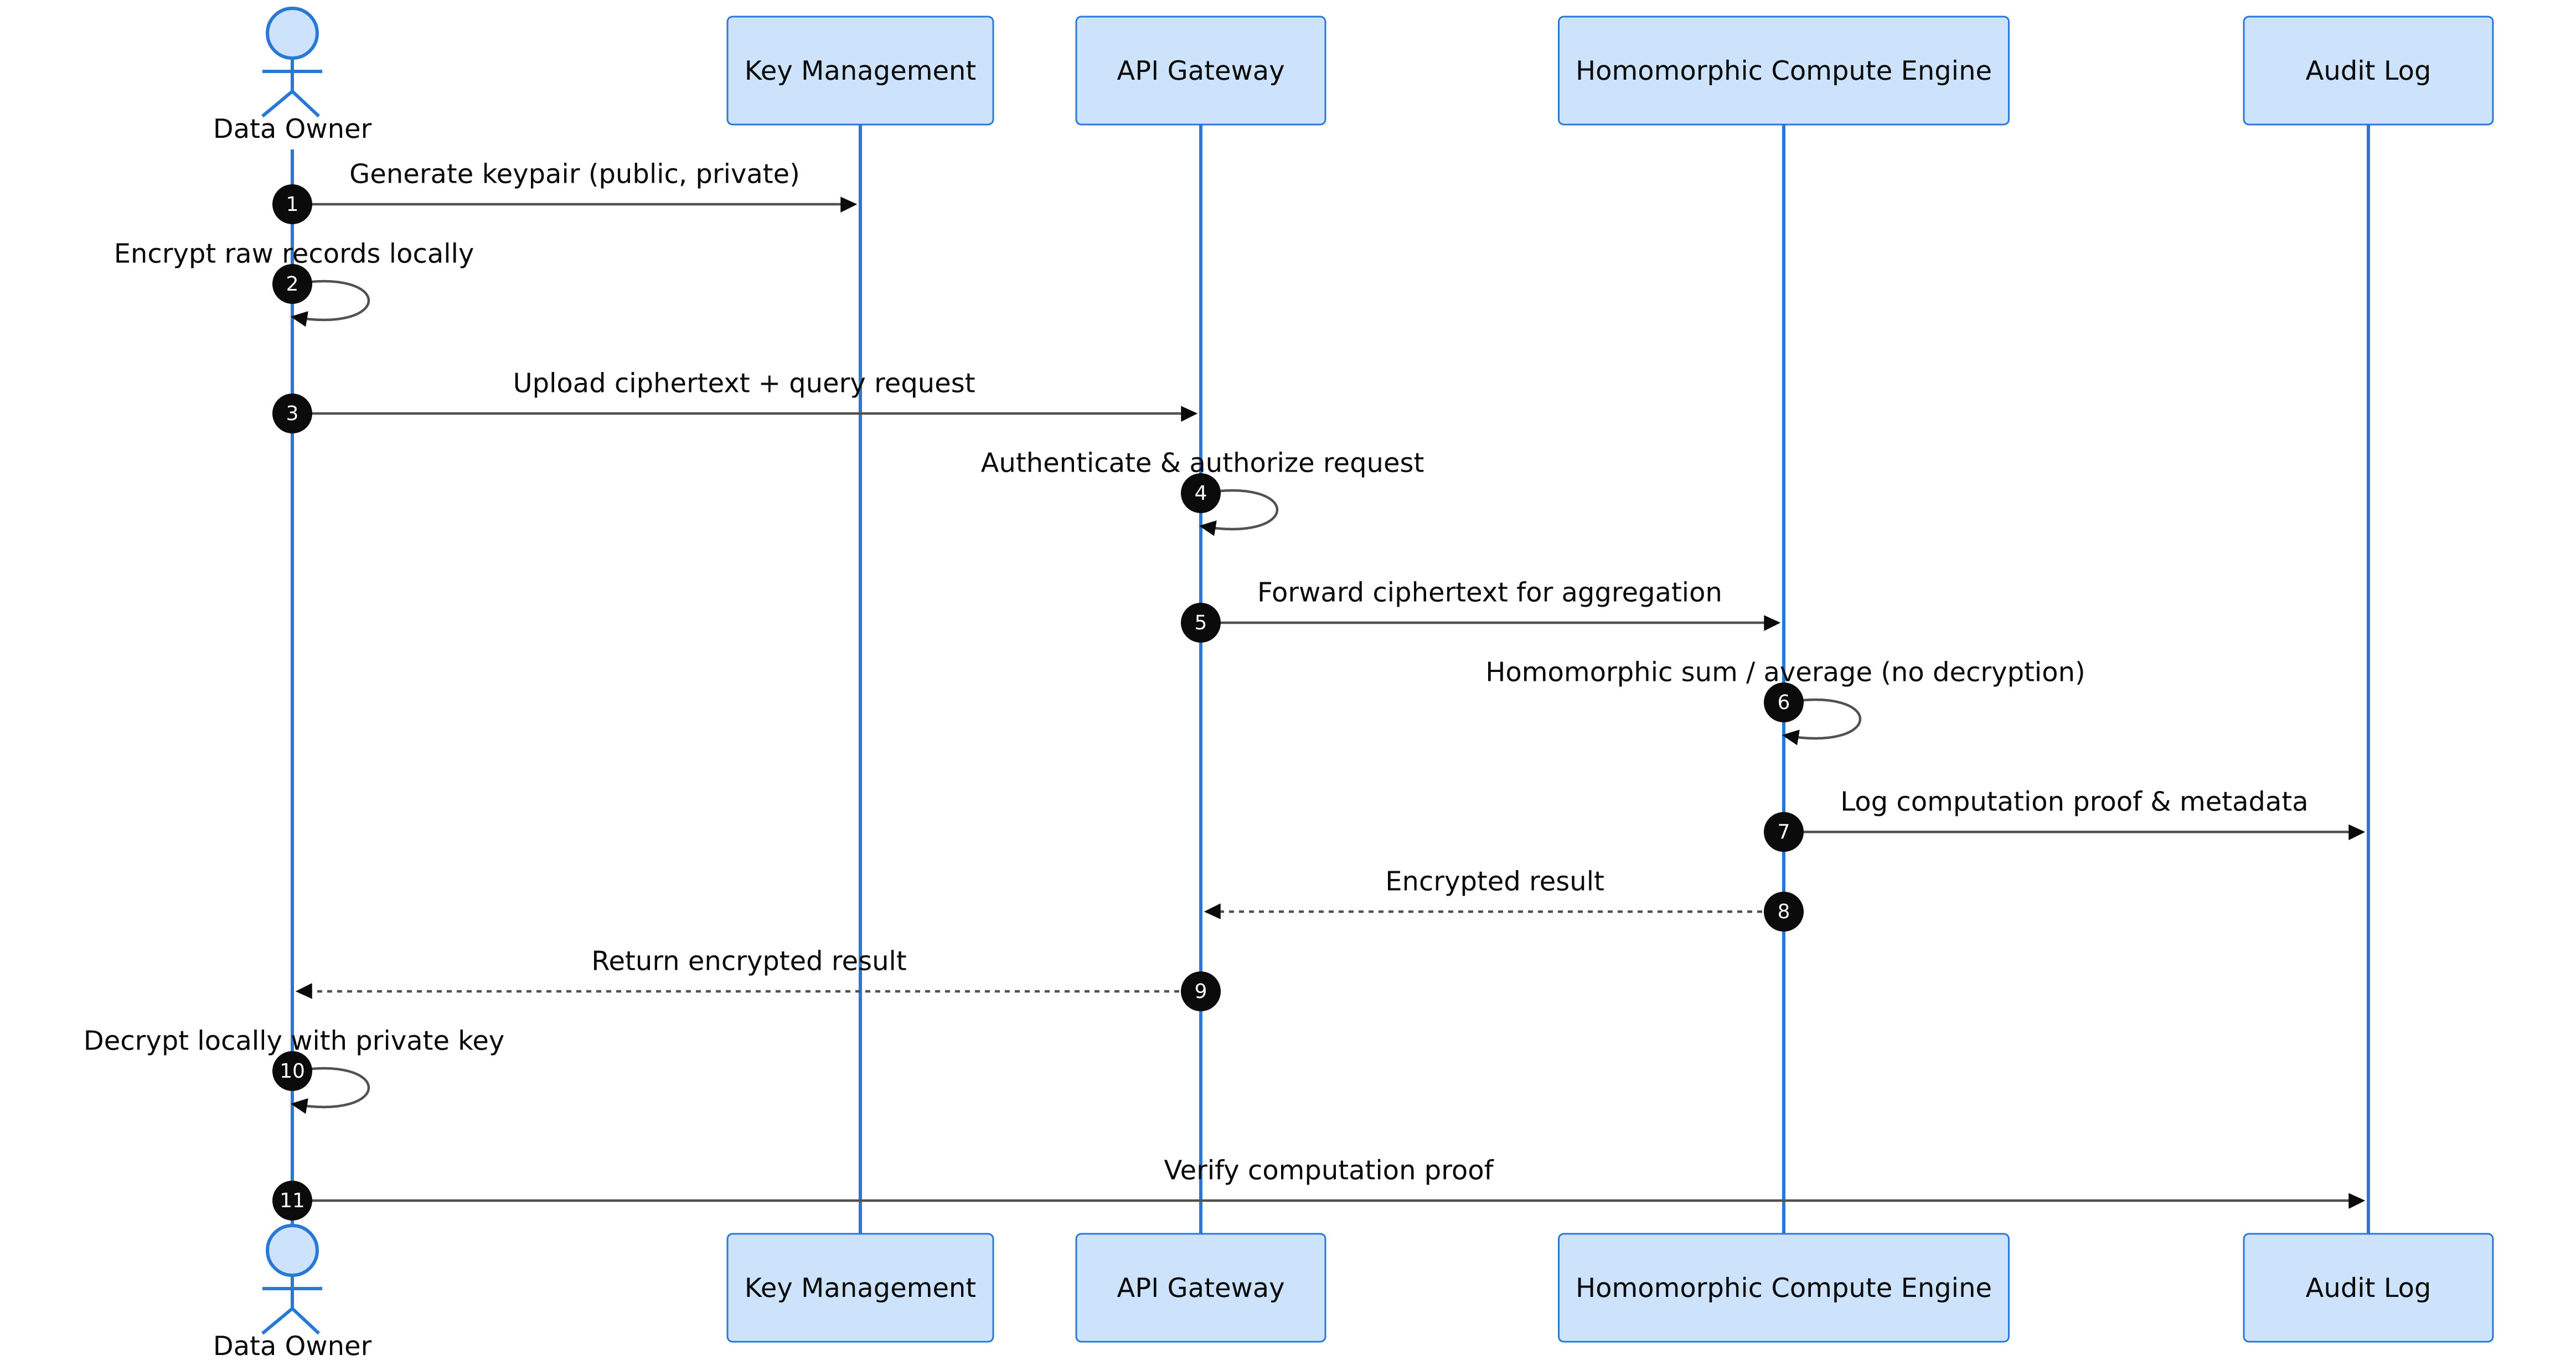
\includegraphics[width=0.85\textwidth]{sources/srs/data-flow-sequence.png}
    \caption{Sequence of operations for a homomorphic aggregation query.}
    \label{fig:data_flow}
\end{figure}

\section{Functional Requirements}

\begin{table}[H]
\centering
\begin{tabularx}{\textwidth}{l l X}
\toprule
\textbf{ID} & \textbf{Requirement} & \textbf{Description} \\
\midrule
FR-1 & Local Key Generation & The Data Owner client must generate a Paillier (or equivalent additively homomorphic) keypair locally; the private key must never leave the trusted domain. \\
FR-2 & Client-Side Encryption & Raw records must be encrypted on the Data Owner's infrastructure before any network transmission. \\
FR-3 & Homomorphic Aggregation & The cloud engine must compute sum, average, and count directly over ciphertext without decryption, using additive homomorphism and plaintext-scalar multiplication. \\
FR-4 & Access Control \& Policy Engine & The API Gateway must authenticate and authorize every query request against a role-based policy before ciphertext is released to the compute engine. \\
FR-5 & Result Return \& Local Decryption & Aggregated encrypted results must be returned to the Data Owner and decrypted only within the trusted domain. \\
FR-6 & Verifiable Computation Log & Every computation must emit an auditable, tamper-evident log entry (operation type, input ciphertext hashes, timestamp) so the Data Owner can verify correctness. \\
FR-7 & Multi-Key-Length Support & The Engine must support configurable key bit-lengths (at minimum 1024/2048/3072) so operators can trade off security margin against latency. \\
FR-8 & Admin Monitoring Dashboard & Operators must be able to observe query throughput, latency, and storage consumption without access to any private key or plaintext. \\
\bottomrule
\end{tabularx}
\caption{Functional Requirements}
\label{tab:functional_reqs}
\end{table}

\subsection{Requirement Prioritization}
Figure~\ref{fig:priority} maps each functional requirement against implementation effort and business impact, informing the phased delivery plan: homomorphic aggregation and local key management are the two ``must-ship-first'' capabilities, since every other requirement depends on them.

\begin{figure}[H]
    \centering
    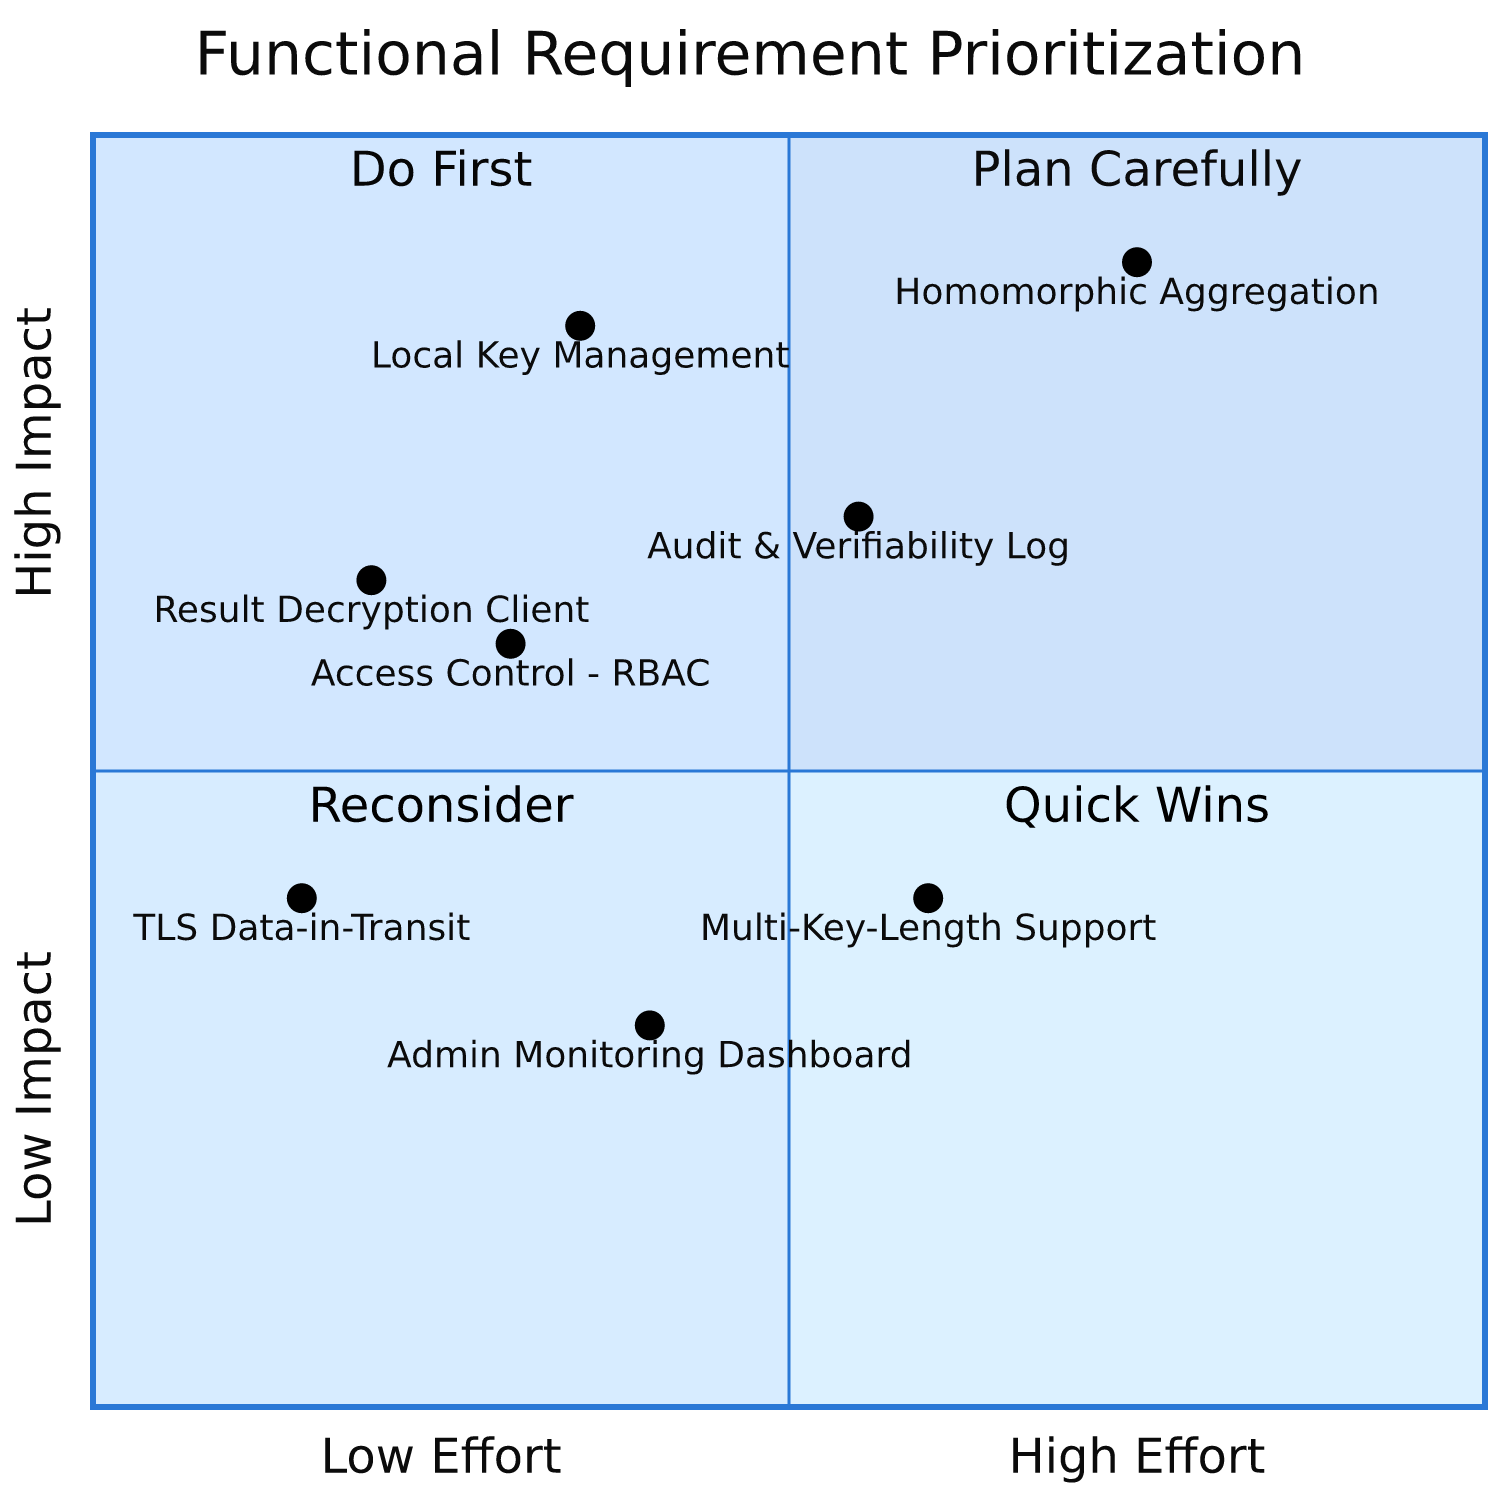
\includegraphics[width=0.75\textwidth]{sources/srs/requirements-priority.png}
    \caption{Functional requirement prioritization by impact vs. implementation effort.}
    \label{fig:priority}
\end{figure}

\section{Non-Functional Requirements}

\begin{table}[H]
\centering
\begin{tabularx}{\textwidth}{l X}
\toprule
\textbf{Category} & \textbf{Requirement} \\
\midrule
Confidentiality & No plaintext sensitive value may exist outside the Data Owner's trusted domain at any point in the pipeline. \\
Integrity \& Verifiability & Every cloud-side computation must be independently verifiable against the audit log; unauthorized modification of stored ciphertext must be detectable (e.g. via authenticated encryption / MAC on ciphertext blobs). \\
Performance & Analytics latency must remain within an operator-configured SLA per key length; based on the empirical study (Section~5), a 2048-bit PHE deployment should target sub-5-minute aggregation latency for a 2M-record batch. \\
Scalability & The compute engine must horizontally scale ciphertext summation across worker nodes, since Paillier summation is embarrassingly parallel. \\
Storage Efficiency & Ciphertext storage expansion must be bounded and predictable; based on Section~5, PHE at 2048-bit keys is budgeted at $\leq$ 1.1 GB per 100 MB of plaintext (an $\sim$11x expansion), versus FHE's $\sim$650x. \\
Availability & The API Gateway and compute engine must meet a 99.5\% uptime target, independent of the Data Owner's local infrastructure availability. \\
Auditability & All access-control decisions and computations must be logged with sufficient metadata for post-hoc compliance review (e.g. HIPAA, GDPR-style audits), without logging plaintext. \\
Usability & The client-side encryption/decryption library must expose a single-call API (encrypt/aggregate/decrypt) so integration effort for a new Data Owner is under one engineer-week. \\
\bottomrule
\end{tabularx}
\caption{Non-Functional Requirements}
\label{tab:nonfunctional_reqs}
\end{table}

\section{Empirical Justification of Cryptographic Scheme Selection}

To ground the Engine's design in evidence rather than assumption, the Feasibility and Computation Overhead studies benchmarked four candidate approaches -- \textbf{Plaintext} (baseline), \textbf{RSA} (decrypt-compute-re-encrypt), \textbf{PHE / Paillier} (additive homomorphism), and \textbf{FHE / TenSEAL CKKS} (arbitrary homomorphism) -- across key lengths of 1024, 2048, and 3072 bits, extrapolated from a 1{,}000-record sample to the full 2{,}000{,}000-record / 94.76~MB financial dataset (a 2000x scale factor).

\subsection{Storage Footprint}
Figure~\ref{fig:storage} shows that FHE ciphertext expansion is catastrophic for tabular aggregation workloads (up to 617~GB for a 94.76~MB source file, a $\sim$6{,}600x expansion), while PHE remains within a manageable $\sim$11--16x expansion across all tested key lengths.

\begin{figure}[H]
    \centering
    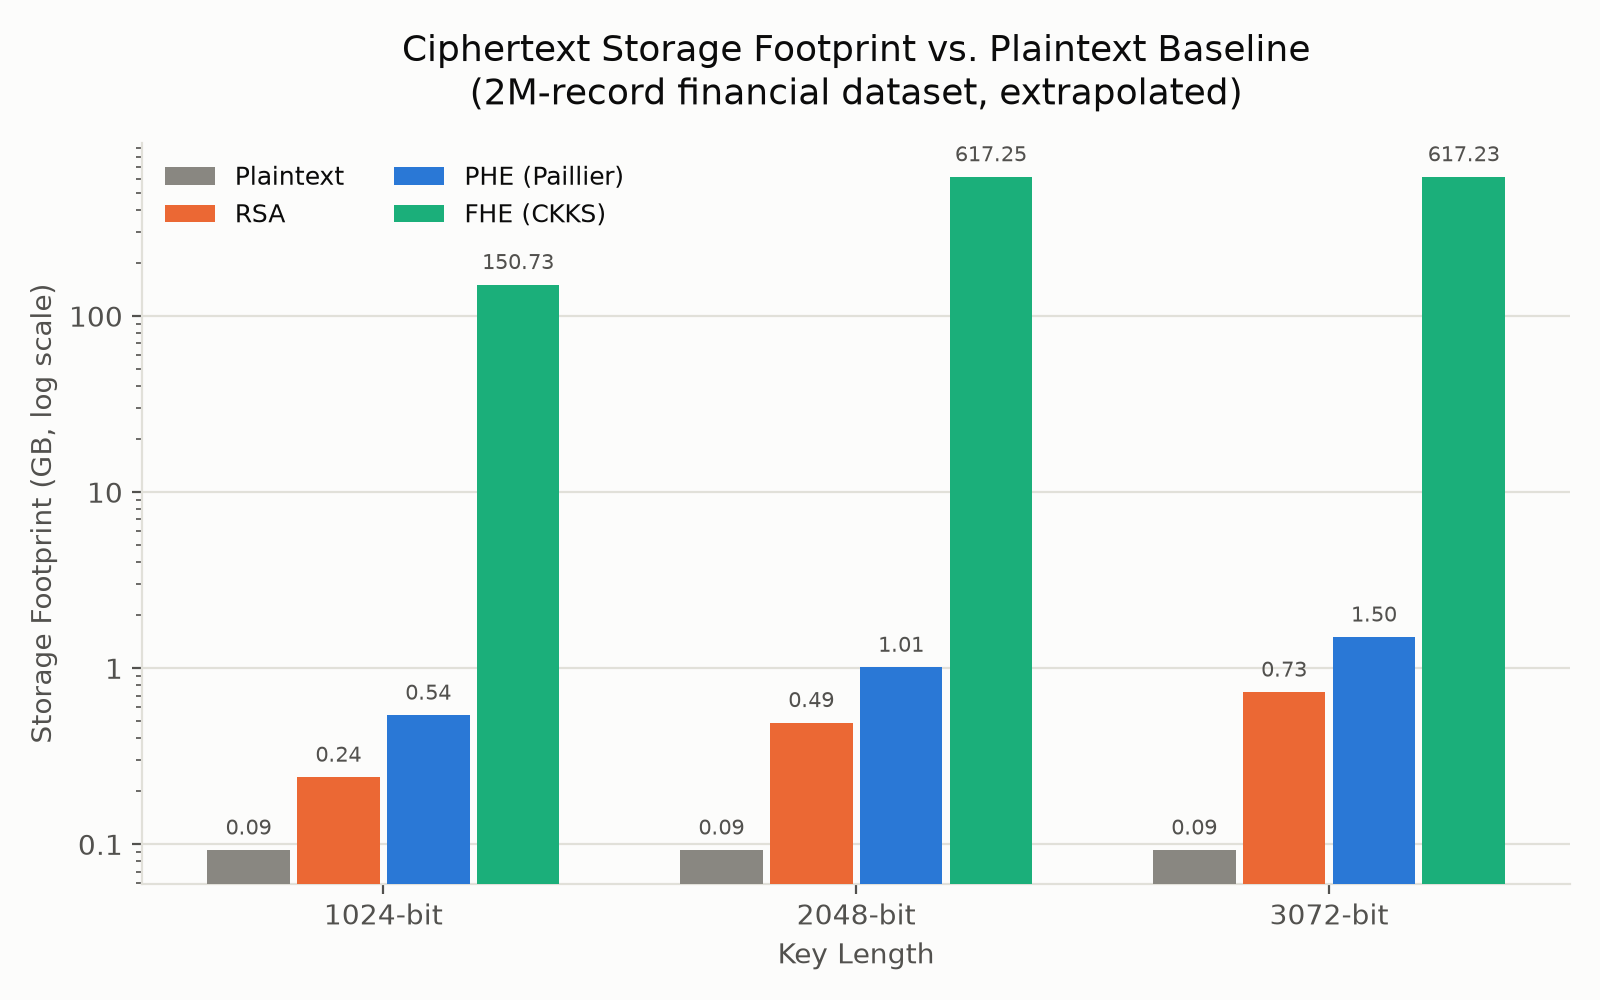
\includegraphics[width=0.85\textwidth]{sources/srs/chart-storage-footprint.png}
    \caption{Ciphertext storage footprint by cryptographic scheme and key length (log scale).}
    \label{fig:storage}
\end{figure}

\subsection{Encryption Latency}
Figure~\ref{fig:enc_latency} shows the full-dataset encryption latency. PHE encryption is the slowest to \emph{ingest} at higher key lengths (112 hours at 3072-bit), which drives NFR guidance to default to 2048-bit keys and to parallelize/pipeline ingestion rather than block on full-dataset encryption before any query can run.

\begin{figure}[H]
    \centering
    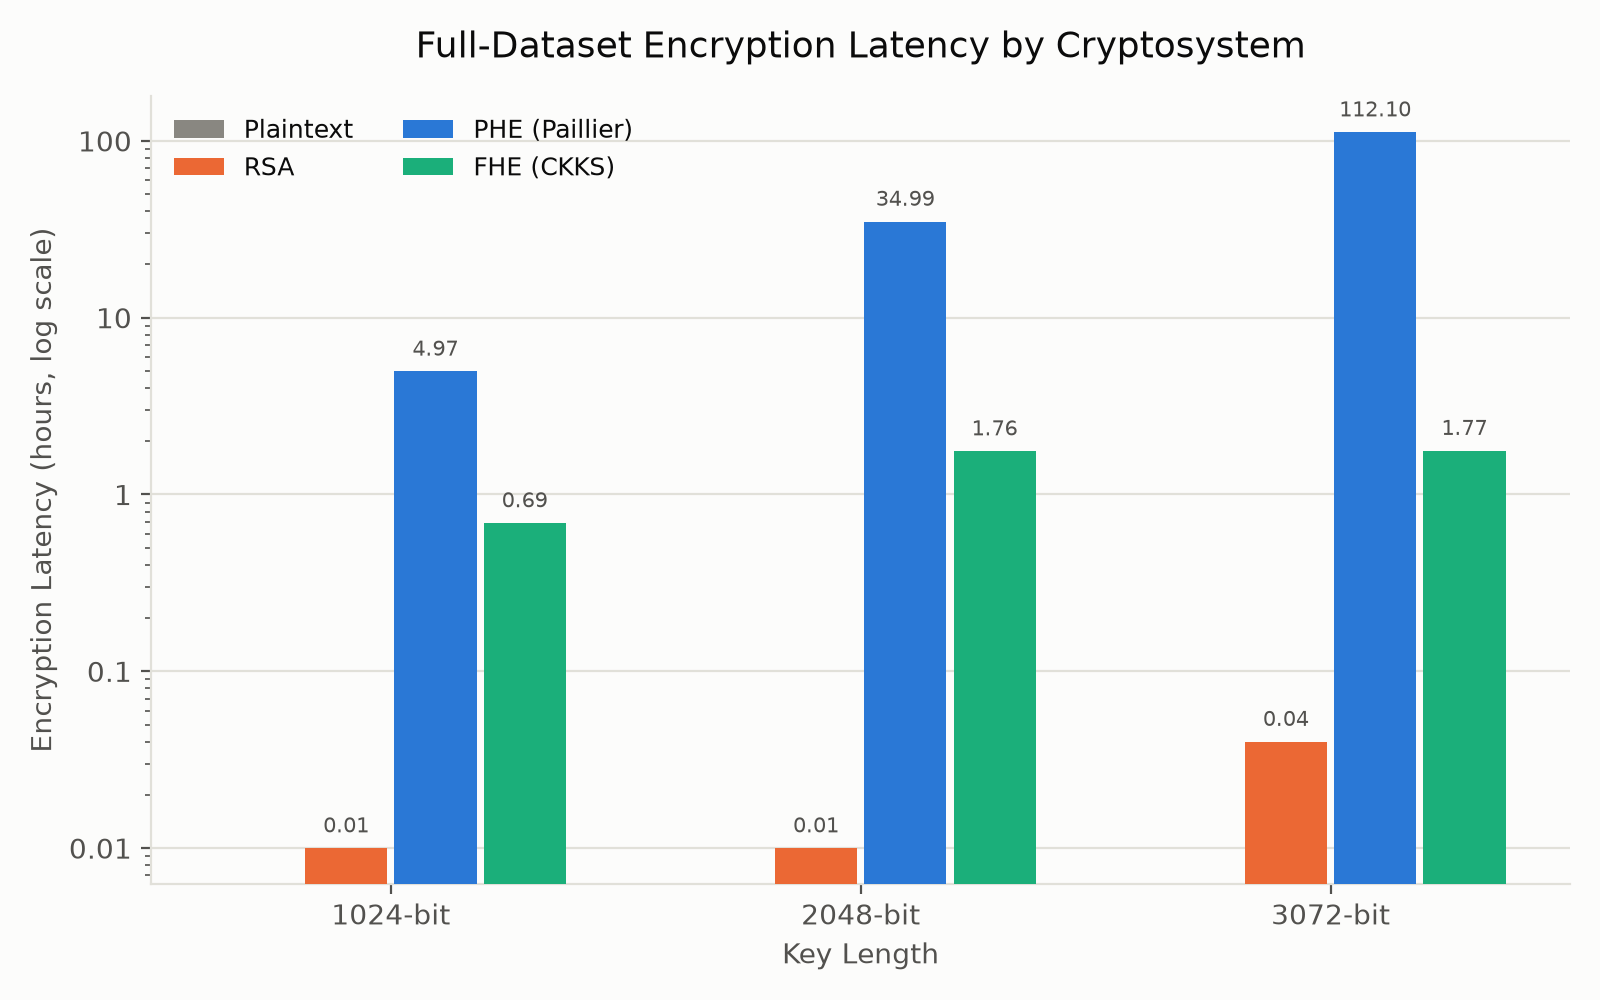
\includegraphics[width=0.85\textwidth]{sources/srs/chart-encryption-latency.png}
    \caption{Full-dataset encryption latency by cryptographic scheme and key length (log scale).}
    \label{fig:enc_latency}
\end{figure}

\subsection{Analytics (Query) Latency}
Figure~\ref{fig:analytics_latency} shows the latency of the actual sum/average computation on already-encrypted data -- the metric that dominates user-perceived query responsiveness. PHE outperforms both RSA's decrypt-compute-re-encrypt pipeline (which additionally violates the Data-in-Use confidentiality requirement) and FHE at every key length tested.

\begin{figure}[H]
    \centering
    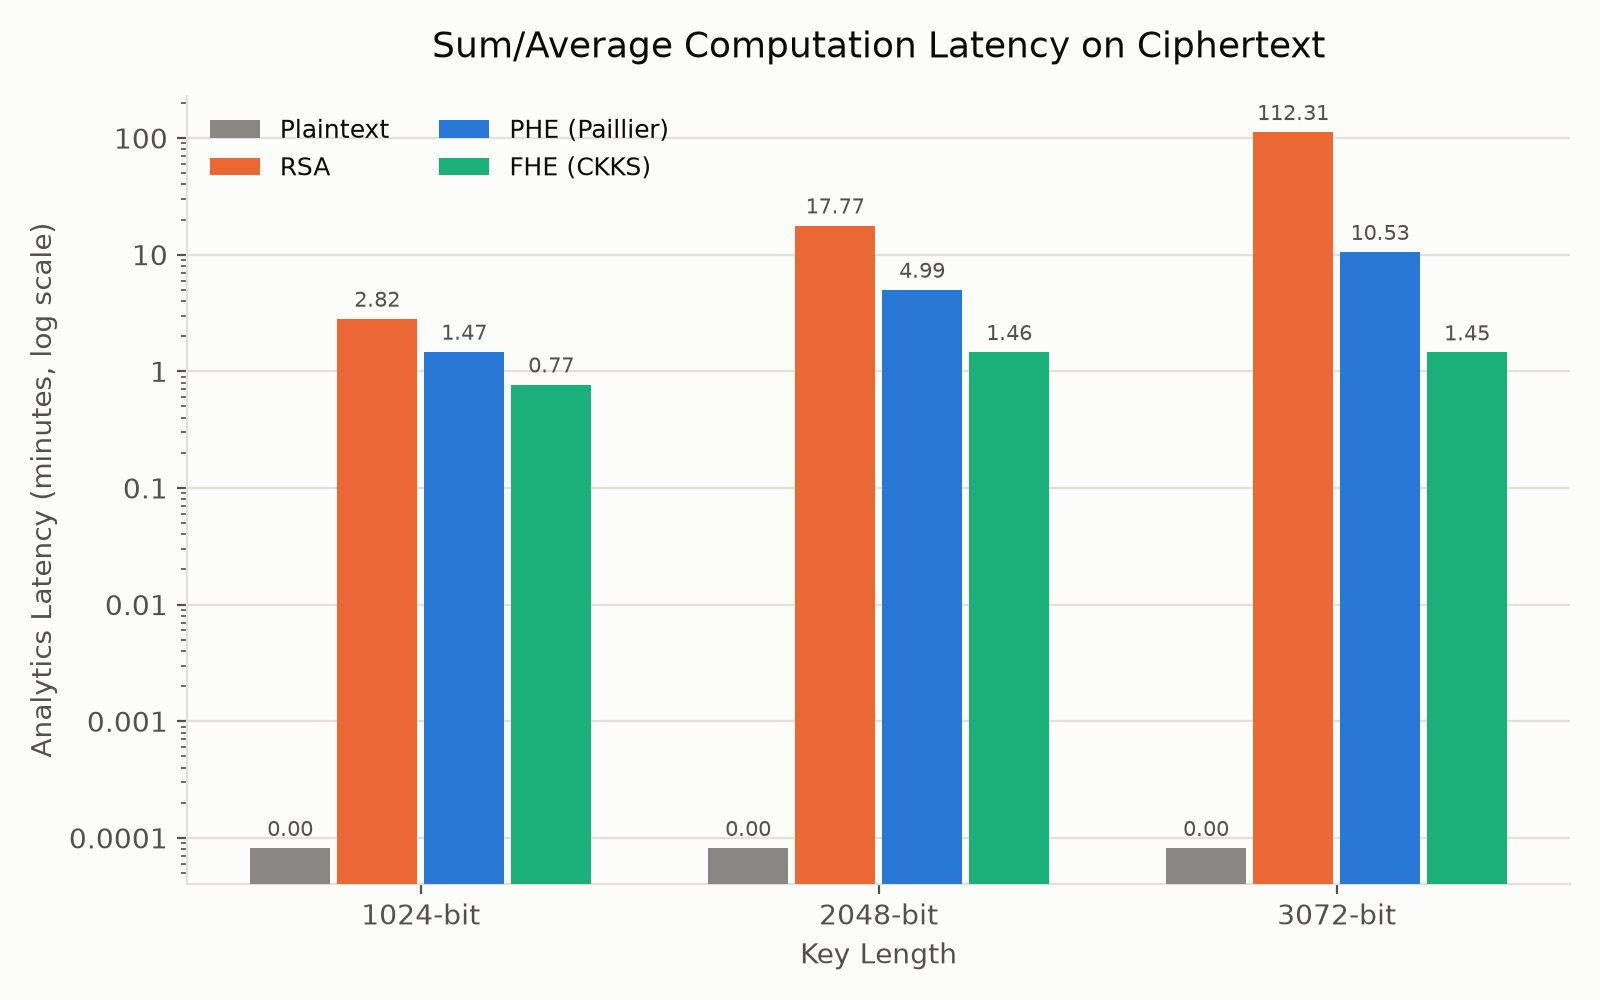
\includegraphics[width=0.85\textwidth]{sources/srs/chart-analytics-latency.png}
    \caption{Ciphertext sum/average computation latency by cryptographic scheme and key length (log scale).}
    \label{fig:analytics_latency}
\end{figure}

\subsection{Trade-off Synthesis}
Figure~\ref{fig:tradeoff} plots storage footprint against analytics latency for the three encrypted schemes. PHE occupies the most favorable region of the trade-off space -- low storage expansion \emph{and} low query latency -- for additive aggregation workloads, whereas FHE's generality is paid for with orders-of-magnitude worse storage and no corresponding analytics-latency benefit for this workload class.

\begin{figure}[H]
    \centering
    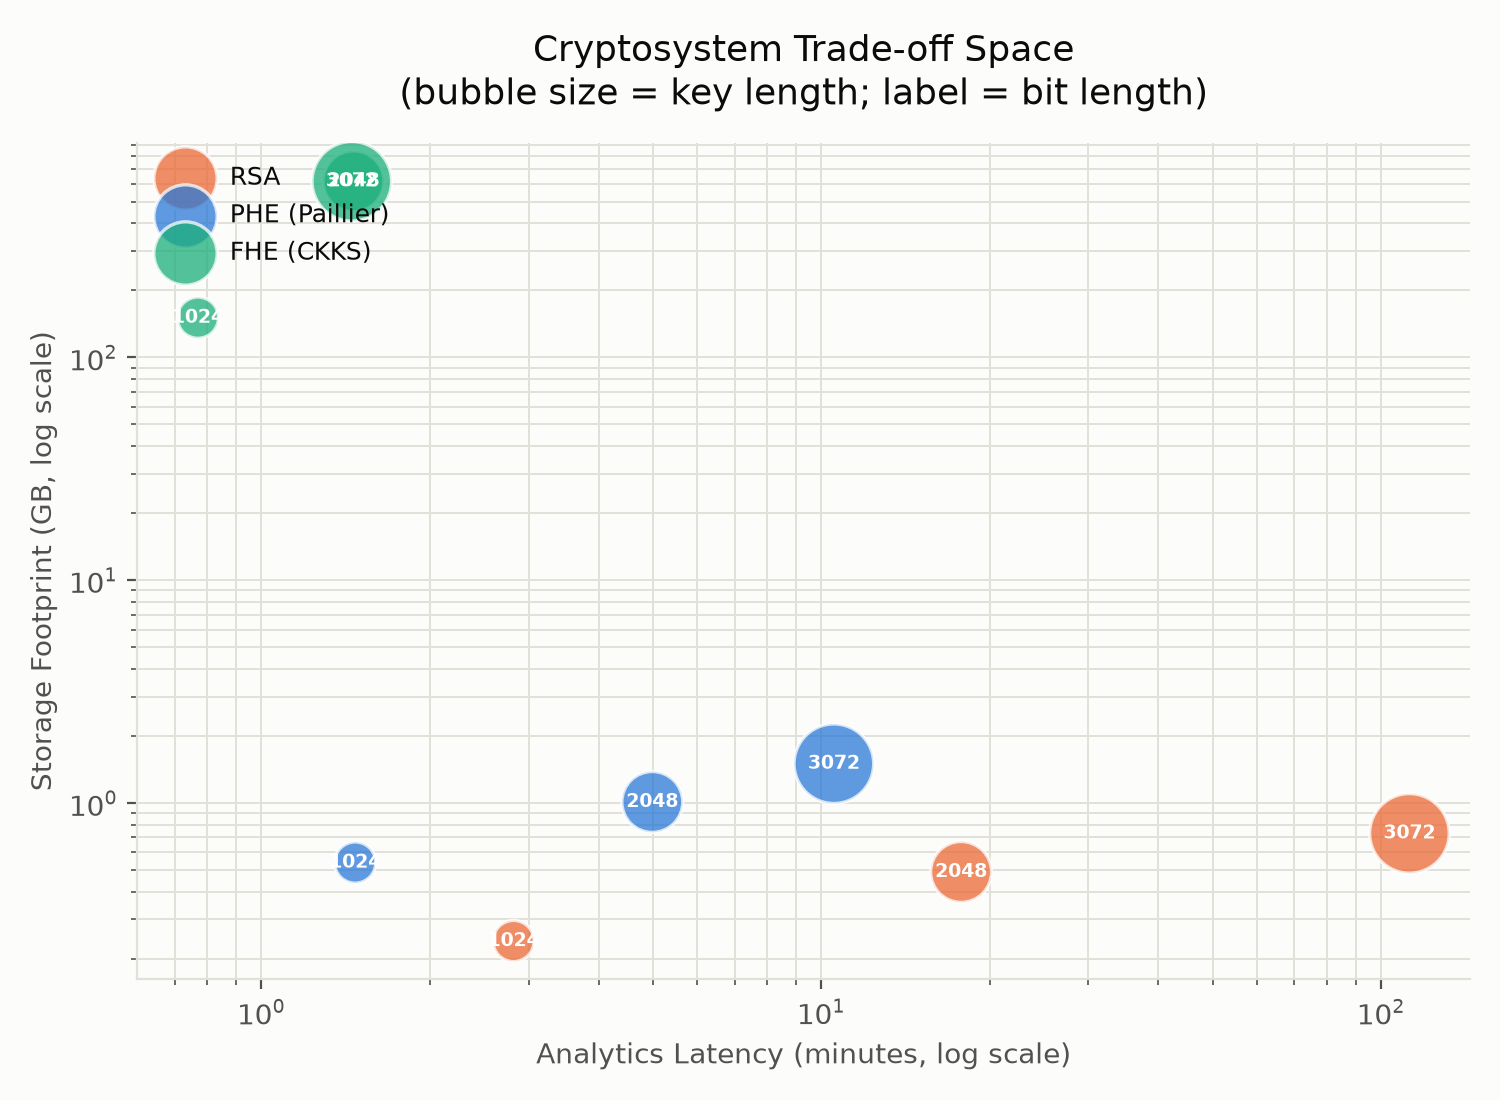
\includegraphics[width=0.8\textwidth]{sources/srs/chart-tradeoff-scatter.png}
    \caption{Storage footprint vs. analytics latency trade-off space across cryptosystems and key lengths.}
    \label{fig:tradeoff}
\end{figure}

\subsection{Decision}
Based on this empirical evidence, the Engine's \textbf{Homomorphic Computation Engine (FR-3) is specified around Partially Homomorphic Encryption (Paillier)} at a default 2048-bit key length, matching the industry-standard security margin while keeping storage expansion and analytics latency within operationally acceptable bounds. FHE (CKKS) is retained as a \emph{pluggable future option} (per A1) for workloads that require multiplicative operations between two ciphertexts, which Paillier does not support.

\section{Requirements Traceability}

\begin{table}[H]
\centering
\begin{tabularx}{\textwidth}{l X l}
\toprule
\textbf{Security Requirement} & \textbf{Addressed By} & \textbf{Req. ID} \\
\midrule
Confidentiality & Client-side encryption; no server-side decryption ever occurs & FR-1, FR-2, FR-3 \\
Integrity & Tamper-evident audit log; authenticated ciphertext storage & FR-6 \\
Anonymity & Aggregation-only query surface prevents record-level linkage; direct identifiers never leave the trusted domain & FR-2, FR-4 \\
Verifiability & Verifiable computation log independently checkable by the Data Owner & FR-6 \\
\bottomrule
\end{tabularx}
\caption{Traceability from security requirements to functional requirements.}
\label{tab:traceability}
\end{table}

\section{Constraints and Future Work}
\begin{itemize}[leftmargin=1.5em]
    \item Paillier's lack of native ciphertext-ciphertext multiplication limits the Engine to linear aggregate statistics in this phase; variance/standard-deviation queries require either a two-round protocol or a partial FHE fallback.
    \item Encryption latency at higher key lengths (Figure~\ref{fig:enc_latency}) motivates a streaming/incremental ingestion pipeline rather than a batch-encrypt-then-query model, to be detailed in the subsequent design deliverable.
    \item Multi-owner federated queries and differential-privacy noise injection for output perturbation are explicitly deferred (A2, A1) and should be scoped in a follow-on SRS revision.
\end{itemize}

\section{Conclusion}
This SRS specifies a concrete, empirically justified system design for privacy-preserving analytics. By confining plaintext exclusively to the Data Owner's trusted domain and performing all cloud-side analytics via Partially Homomorphic Encryption, the Engine closes the Data-in-Use vulnerability window while remaining within practical storage and latency budgets, as demonstrated by the benchmarking data in Section~5.

\end{document}
